% Runtime-Adaptive Sparse Matrix Optimization for GPUs (RASP): sequential implementation, hotspots and choice of
% platform (five slides + title). Build: latexmk -pdf hotspots.tex
% Every number and chart comes from scripts/analyze_seq.py (generated/seq.tex, generated/*.csv) or the Phase 0 probe
% (../../report/generated/platform.tex); edit the team block below, not the numbers.
\documentclass[aspectratio=169,10pt]{beamer}

\usepackage[T1]{fontenc}
\usepackage{lmodern}
\usepackage{graphicx}
\usepackage{tikz}
\usetikzlibrary{positioning,arrows.meta,calc}
\usepackage{pgfplots}
\usepackage{pgfplotstable}
\pgfplotsset{compat=1.18}
\usepackage{booktabs}
\usepackage{colortbl}
\usepackage{tabularx}

% ---- Theme ----
\usetheme{default}
\useoutertheme{miniframes}
\setbeamertemplate{navigation symbols}{}
\setbeamertemplate{blocks}[rounded][shadow=false]

% ---- Colors ----
\definecolor{accent}{RGB}{5, 102, 141}
\definecolor{darkGray}{RGB}{60,60,60}
\definecolor{deepBlack}{RGB}{0,0,0}
\definecolor{accentDark}{RGB}{4,160,120}
\definecolor{softRed}{RGB}{196,64,64}
\definecolor{muted}{RGB}{169,199,214}

\setbeamercolor{footlinecolor}{bg=deepBlack, fg=white}
\setbeamertemplate{footline}
{
\leavevmode
\begin{beamercolorbox}[wd=\paperwidth,ht=3.2ex,dp=1.4ex,leftskip=1em,rightskip=1em plus1fil]{footlinecolor}
\textbf{Runtime-Adaptive Sparse Matrix Optimization for GPUs}
\hfill
\textbf{\insertframenumber{} / \inserttotalframenumber}
\end{beamercolorbox}
}

\setbeamercolor{title}{fg=white,bg=accent}
\setbeamercolor{frametitle}{fg=white,bg=accent}
\setbeamercolor{structure}{fg=accent}
\setbeamercolor{item}{fg=accent}
\setbeamercolor{section in head/foot}{fg=white,bg=deepBlack}
\setbeamercolor{subsection in head/foot}{fg=white,bg=deepBlack}
\setbeamercolor{block title}{fg=white,bg=accent}
\setbeamercolor{block body}{fg=darkGray,bg=accent!6}
\setbeamercolor{normal text}{fg=darkGray}

\setbeamerfont{title}{size=\LARGE,series=\bfseries}
\setbeamerfont{frametitle}{size=\Large,series=\bfseries}
\setbeamerfont{block title}{size=\small,series=\bfseries}

% ---- Team (fill in roll numbers / guide; empty fields are not shown) ----
\newcommand{\memberA}{Harsh Raj}\newcommand{\rollA}{S20240010084}
\newcommand{\memberB}{Karmanya}\newcommand{\rollB}{S20240010108}
\newcommand{\memberC}{Vivian}\newcommand{\rollC}{S20240010258}
\newcommand{\guide}{}
\newcommand{\member}[2]{\begin{tabular}[t]{c}\large\textbf{#1}\if\relax\detokenize\expandafter{#2}\relax\else\\[-1pt]{\small (#2)}\fi\end{tabular}}

\setbeamertemplate{title page}
{
    \begin{center}
    \vspace{0.3cm}
    \begin{beamercolorbox}[wd=\paperwidth,sep=12pt,center]{frametitle}
        {\usebeamerfont{title}\inserttitle}\\[4pt]
        {\large\insertsubtitle}
    \end{beamercolorbox}

    \vspace{0.7cm}

    \member{\memberA}{\rollA}\hspace{1.2cm}\member{\memberB}{\rollB}\hspace{1.2cm}\member{\memberC}{\rollC}

    \vspace{0.5cm}

    \if\relax\detokenize\expandafter{\guide}\relax\else
    Under the guidance of\\[2pt]
    \textbf{\guide}

    \vspace{0.4cm}
    \fi

    High Performance Computing \textperiodcentered{} Project Checkpoint\\[2pt]
    {\small Sequential implementation, hotspots and choice of platform}

    \vspace{0.3cm}
    \insertdate

    \vspace{0.35cm}
    {\scriptsize\color{gray}
    M.~Deveci et al., \emph{Sparse Matrix-Matrix Multiplication on Multilevel Memory Architectures}, arXiv:1804.00695
    (2018)\\
    M.~Heller, T.~Oberhuber, \emph{Adaptive Row-grouped CSR Format for Storing of Sparse Matrices on GPU},
    arXiv:1203.5737 (2012)\par}
    \end{center}
}

\title[Runtime-Adaptive Sparse Matrix Optimization for GPUs]{\textbf{Runtime-Adaptive Sparse Matrix\\Optimization for GPUs}}
\subtitle{Sparse matrix representation and GPU memory-layout optimization}
\date{9 October 2026}
\IfFileExists{logo.png}{\logo{\includegraphics[height=1.0cm]{logo.png}}}{}

% ---- Numbers ----
% Report macros. Every result in the report is a \stat{key}: generated/*.tex (scripts/make_report_assets.py) defines
% the values with \setstat{key}{value}. A key without a value prints a red ??key and a LaTeX warning, so a number that
% has not been measured yet (Phases 4-5 before the GPU runs) is impossible to miss.
\makeatletter
\newcommand{\setstat}[2]{\expandafter\def\csname rasp@stat@#1\endcsname{#2}}
\DeclareRobustCommand{\stat}[1]{%
  \ifcsname rasp@stat@#1\endcsname\csname rasp@stat@#1\endcsname
  \else\textcolor{red}{\textbf{??#1}}\PackageWarning{rasp}{No value for `#1' (run scripts/make_report_assets.py)}\fi}
\newcommand{\stattable}[1]{\stat{table:#1}}
% \rfig[width]{name}: figures/name.pdf (or .png), or a visible placeholder until the figure exists.
\newcommand{\rfig}[2][\linewidth]{%
  \IfFileExists{figures/#2.pdf}{\includegraphics[width=#1]{figures/#2.pdf}}{%
    \IfFileExists{figures/#2.png}{\includegraphics[width=#1]{figures/#2.png}}{%
      \fbox{\parbox[c][3.5cm][c]{\dimexpr#1-2\fboxsep-2\fboxrule\relax}{\centering
        \textcolor{red}{\textbf{missing figure: \texttt{\detokenize{#2}}}}\\[2pt]
        \small (produced by \texttt{scripts/make\_report\_assets.py} after the GPU runs)}}}}}
\makeatother
\newcommand{\x}{$\times$}
\newcommand{\G}[1]{\textbf{G#1}}
\newcommand{\todo}[1]{\textcolor{orange}{[TODO: #1]}}

\InputIfFileExists{../../report/generated/platform.tex}{}{}
\InputIfFileExists{generated/seq.tex}{}{}
\newcommand{\statnum}[1]{\csname rasp@stat@#1\endcsname}  % expandable, for drawing and arithmetic
\pgfmathtruncatemacro{\gpuratio}{round(\statnum{pf-device-read}/\statnum{seq-bw-1})}  % GPU vs one core
\newcommand{\yes}{\colorbox{accentDark}{\makebox[2.2em]{\textcolor{white}{\scriptsize\bfseries YES}}}}
\newcommand{\no}{\colorbox{softRed}{\makebox[2.2em]{\textcolor{white}{\scriptsize\bfseries NO}}}}
\newcommand{\aside}[1]{{\color{gray}\scriptsize #1}}
% \callout{text}: a tinted box exactly as wide as the column.
\newcommand{\callout}[1]{\begin{tikzpicture}\node[fill=accent!6, rounded corners=3pt, inner sep=6pt,
  text width=\linewidth-12pt, minimum height=1.25cm, align=left, font=\small, text=darkGray]{#1};\end{tikzpicture}}
\newcommand{\charttitle}[2]{{\small\bfseries #1}\\[-1pt]{\scriptsize\color{gray}#2}\par}

% ---- Charts (pgfplots: same font and colours as the slides) ----
\pgfplotsset{
  table/col sep=comma,
  /pgf/number format/assume math mode=true,  % value labels in the text font, so they can be bold
  hbars/.style={
    xbar, bar shift=0pt, bar width=6.5pt, scale only axis, clip=false, xmin=0,
    axis x line=none, axis y line=left, y axis line style={draw=none}, ytick=data, ytick style={draw=none},
    y tick label style={font=\scriptsize, text=darkGray}, enlarge y limits={abs=0.55},
  },
  valuelabels/.style={
    only marks, mark=none, point meta=x,
    every node near coord/.append style={font=\scriptsize\bfseries, text=darkGray, anchor=west, xshift=-1pt},
  },
  swatch legend/.style={legend image code/.code={\fill[##1] (0cm,-0.1cm) rectangle (0.3cm,0.1cm);}},
}
\pgfplotstableset{col sep=comma}
% \gprofpanel{csv}: top-5 functions of one workload, the largest in the accent colour.
\newcommand{\gprofpanel}[1]{%
  \begin{tikzpicture}
  \begin{axis}[hbars, width=2.1cm, height=2.75cm, xmax=58, bar width=7.5pt, yticklabels from table={#1}{label}]
    \addplot[fill=accent, draw=none] table[x=top, y expr=\coordindex]{#1};
    \addplot[fill=muted, draw=none] table[x=rest, y expr=\coordindex]{#1};
    \addplot[valuelabels, nodes near coords={\pgfmathprintnumber[fixed,precision=0]{\pgfplotspointmeta}\%}]
      table[x expr=\thisrow{top}+\thisrow{rest}, y expr=\coordindex]{#1};
  \end{axis}
  \end{tikzpicture}}

\begin{document}

%------------------------------------------------
\begin{frame}[plain,noframenumbering]
\titlepage
\end{frame}

%================================================
\section{Implementation}

\begin{frame}{The Sequential Implementation}

\small
Three workloads in one \textbf{single-threaded C++ program}, profiled to find where the time goes.

\vspace{0.4cm}

\centering
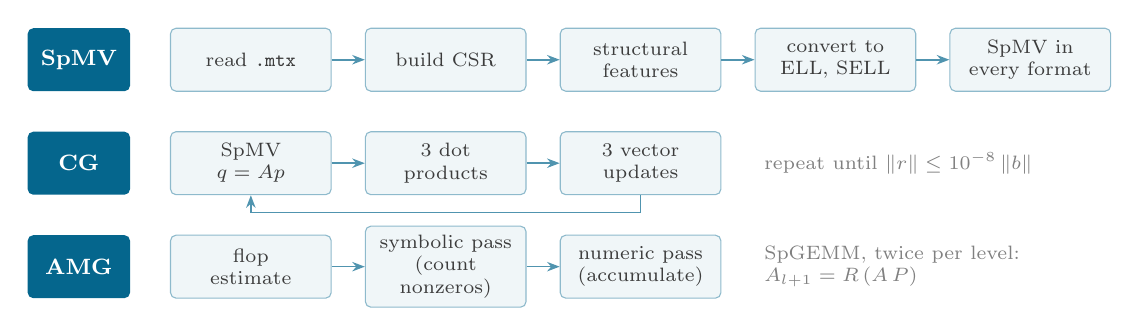
\begin{tikzpicture}[
  stage/.style={draw=accent!45, fill=accent!6, rounded corners=2pt, minimum height=8mm, text width=19mm,
               align=center, font=\scriptsize, text=darkGray, inner xsep=2pt},
  tag/.style={fill=accent, text=white, rounded corners=2pt, minimum height=8mm, minimum width=13mm,
              font=\footnotesize\bfseries},
  arr/.style={-{Stealth[length=1.6mm]}, draw=accent!70, semithick},
  note/.style={font=\scriptsize, text=gray, anchor=west, align=left},
  gap/.style={node distance=4.2mm}]
  % SpMV
  \node[tag] (t1) {SpMV};
  \node[stage, right=5mm of t1] (a1) {read \texttt{.mtx}};
  \node[stage, gap, right=of a1] (a2) {build CSR};
  \node[stage, gap, right=of a2] (a3) {structural\\features};
  \node[stage, gap, right=of a3] (a4) {convert to\\ELL, SELL};
  \node[stage, gap, right=of a4] (a5) {SpMV in\\every format};
  \foreach \a/\b in {a1/a2, a2/a3, a3/a4, a4/a5} \draw[arr] (\a) -- (\b);
  % CG
  \node[tag, below=5mm of t1] (t2) {CG};
  \node[stage, right=5mm of t2] (b1) {SpMV\\\mbox{$q = Ap$}};
  \node[stage, gap, right=of b1] (b2) {3 dot\\products};
  \node[stage, gap, right=of b2] (b3) {3 vector\\updates};
  \foreach \a/\b in {b1/b2, b2/b3} \draw[arr] (\a) -- (\b);
  \draw[arr] (b3.south) -- ++(0,-2.2mm) -| (b1.south);
  \node[note] at (a4.west |- b3) {repeat until $\|r\| \le 10^{-8}\,\|b\|$};
  % AMG
  \node[tag, below=5mm of t2] (t3) {AMG};
  \node[stage, right=5mm of t3] (c1) {flop\\estimate};
  \node[stage, gap, right=of c1] (c2) {symbolic pass\\(count nonzeros)};
  \node[stage, gap, right=of c2] (c3) {numeric pass\\(accumulate)};
  \foreach \a/\b in {c1/c2, c2/c3} \draw[arr] (\a) -- (\b);
  \node[note] at (a4.west |- c3) {SpGEMM, twice per level:\\$A_{l+1} = R\,(A\,P)$};
\end{tikzpicture}

\vspace{0.45cm}
\raggedright
\begin{columns}[T,onlytextwidth]
\column{0.44\textwidth}
\aside{INPUTS}\\
\footnotesize 6 SuiteSparse matrices (0.56M--17.6M nonzeros)\\3-D Laplacian, $128^3$ and $160^3$
\column{0.30\textwidth}
\aside{CODE}\\
\footnotesize \texttt{seq/rasp\_seq.cpp}\\C++17, \texttt{g++ -O2}, no libraries
\column{0.22\textwidth}
\aside{MACHINE}\\
\footnotesize Intel Core i7-1255U\\one core, WSL2
\end{columns}

\end{frame}

%================================================
\section{Profiling}

\begin{frame}{Profiling: Where the Time Goes}

\small
Bars: share of \textbf{gprof} samples per function, top 5 (GCC cloning disabled, so time lands on the right
function). \textbf{getrusage} timers add wall, user and system time per phase.

\vspace{0.4cm}

\begin{columns}[T,onlytextwidth]
\column{0.32\textwidth}
\charttitle{SpMV workload}{6 matrices $\times$ 3 formats, \stat{seq-spmv-total-s}\,s}
\vspace{1mm}
\gprofpanel{generated/gprof_spmv.csv}\\[1mm]
\footnotesize SpMV kernels: \stat{seq-spmv-kernel-pct}\% of wall time. Reading and building CSR happen once.

\column{0.32\textwidth}
\charttitle{CG solver}{Laplace $128^3$, 2.1M rows, \stat{seq-cg-total-s}\,s}
\vspace{1mm}
\gprofpanel{generated/gprof_cg.csv}\\[1mm]
\footnotesize SpMV takes half; the four vector operations take the other half.

\column{0.32\textwidth}
\charttitle{AMG set-up}{Laplace $160^3$, 4.1M rows, \stat{seq-amg-total-s}\,s}
\vspace{1mm}
\gprofpanel{generated/gprof_amg.csv}\\[1mm]
\footnotesize SpGEMM's three passes dominate; the numeric pass alone is half.
\end{columns}

\end{frame}

%================================================
\section{Memory traffic}

\begin{frame}{Why They Are Hot: Memory Traffic}

\begin{columns}[T,onlytextwidth]
\column{0.52\textwidth}
\charttitle{One CG iteration: bytes vs time}{%
  share of the \stat{seq-cg-iter-mb}\,MB moved (model) and of the time (measured)}
\vspace{2mm}
\begin{tikzpicture}
\begin{axis}[xbar, bar width=9pt, scale only axis, width=4.6cm, height=2.5cm, xmin=0, xmax=70, clip=false,
  axis x line=none, axis y line=left, y axis line style={draw=none}, ytick=data, ytick style={draw=none},
  y tick label style={font=\small, text=darkGray}, enlarge y limits={abs=0.7}, y dir=reverse,
  yticklabels from table={generated/cg_traffic.csv}{label},
  nodes near coords={\pgfmathprintnumber[fixed,precision=0]{\pgfplotspointmeta}\%},
  every node near coord/.append style={font=\scriptsize\bfseries, text=darkGray},
  legend style={draw=none, font=\scriptsize, at={(0.5,1.03)}, anchor=south, legend columns=2,
                /tikz/every even column/.append style={column sep=8pt}},
  swatch legend, reverse legend]
  \addplot[fill=accent, draw=none] table[x=time, y expr=\coordindex]{generated/cg_traffic.csv};
  \addplot[fill=muted, draw=none] table[x=bytes, y expr=\coordindex]{generated/cg_traffic.csv};
  \legend{time, bytes moved}
\end{axis}
\end{tikzpicture}

\vspace{2mm}
\small The vector operations do almost no arithmetic, yet take more time than SpMV, because they move more bytes.
\textbf{Time follows bytes, not flops.}

\column{0.44\textwidth}
\begin{block}{SpMV is bandwidth-bound}
\small 2 flops per $\geq$\,12 bytes read. At \stat{seq-bw-1}\,GB/s, one core can do about
\textbf{\stat{seq-spmv-bound-gflops} GFLOP/s}; we measure \stat{seq-csr-gflops-min}--\stat{seq-csr-gflops-max}.
The sequential code already runs at memory speed.
\end{block}
\vspace{1mm}
\begin{block}{SpGEMM pays for memory too}
\small \textbf{\stat{seq-amg-numeric-sys-pct}\%} of the numeric pass is system time: the OS zero-filling freshly
allocated output pages. gprof cannot see this; getrusage can.
\end{block}
\end{columns}

\end{frame}

%================================================
\section{Parallelism}

\begin{frame}{Can the Hotspots Run in Parallel?}

\vspace{0.15cm}
\footnotesize
\renewcommand{\arraystretch}{1.6}
\begin{tabularx}{\textwidth}{@{}l c l X@{}}
\toprule
\textbf{Hotspot} & \textbf{Parallel?} & \textbf{Pattern} & \textbf{The catch} \\
\midrule
SpMV & \yes & map over rows & uneven rows: the format must fit \\
Dot products & \yes & reduction & per-thread partial sums, combined in a tree \\
axpy, Jacobi, $p$-update & \yes & map over entries & none: limited only by bandwidth \\
SpGEMM, both passes & \yes & map over rows of $C$ & size of $C$ unknown: count first, then fill \\
Flop estimate, ELL/SELL build & \yes & map + prefix sum & the prefix sum becomes a parallel scan \\
\rowcolor{softRed!7}
CG iteration loop & \no & sequential in $k$ & step $k{+}1$ needs $\alpha_k$ and $\beta_k$ from step $k$ \\
\rowcolor{softRed!7}
Reading \texttt{.mtx} & \no & sequential I/O & runs once per matrix: store a binary CSR \\
\bottomrule
\end{tabularx}

\vspace{0.4cm}
\small Everything that takes real time is a \textbf{map} or a \textbf{reduction} over millions of independent rows:
the work GPUs are built for. The CG loop stays sequential; each step inside it runs in parallel.

\end{frame}

%================================================
\section{Platform}

\begin{frame}{Platform: CUDA}

\begin{columns}[T,onlytextwidth]
\column{0.47\textwidth}
\charttitle{Memory bandwidth, measured}{streaming read on the CPU, device read on the GPU}
\vspace{2mm}
\begin{tikzpicture}
\begin{axis}[hbars, width=2.8cm, height=1.7cm, xmax=\statnum{pf-device-read}, bar width=9pt,
  ytick={0,1,2}, yticklabels={1 CPU core, \statnum{seq-bw-threads} CPU threads, RTX 4050 GPU},
  y tick label style={font=\footnotesize}]
  \addplot[fill=muted, draw=none] coordinates {(\statnum{seq-bw-1},0) (\statnum{seq-bw-all},1)};
  \addplot[fill=accent, draw=none] coordinates {(\statnum{pf-device-read},2)};
  \addplot[valuelabels, nodes near coords={\pgfmathprintnumber[fixed,precision=1]{\pgfplotspointmeta}\,GB/s}]
    coordinates {(\statnum{seq-bw-1},0) (\statnum{seq-bw-all},1) (\statnum{pf-device-read},2)};
\end{axis}
\end{tikzpicture}

\vspace{2mm}
\small Memory-bound code runs at memory speed: the GPU has \textbf{\gpuratio\x} one core's bandwidth, and thousands of
threads to hide irregular reads.

\column{0.47\textwidth}
\charttitle{SpMV: GPU over sequential, \stat{seq-gpu-speedup-geomean}\x{} geomean}{cuSPARSE on the RTX 4050 vs our
  CSR on one core}
\vspace{2mm}
\begin{tikzpicture}
\begin{axis}[hbars, width=3.1cm, height=2.35cm, xmax=17, bar width=6.5pt,
  yticklabels from table={generated/speedup.csv}{label}]
  \addplot[fill=accent, draw=none] table[x=ratio, y expr=\coordindex]{generated/speedup.csv};
  \addplot[valuelabels, nodes near coords={\pgfmathprintnumber[fixed,precision=1]{\pgfplotspointmeta}$\times$}]
    table[x=ratio, y expr=\coordindex]{generated/speedup.csv};
\end{axis}
\end{tikzpicture}

\aside{Preliminary: CPU and GPU are on different laptops.}
\end{columns}

\vspace{0.35cm}
\begin{columns}[T,onlytextwidth]
\column{0.47\textwidth}
\callout{\textbf{\color{accent}Not OpenMP alone:} \stat{seq-bw-threads} threads give only \stat{seq-bw-scaling}\x,
  because they share one memory bus.}
\column{0.47\textwidth}
\callout{\textbf{\color{accent}Not MPI:} one node is enough. Data larger than the GPU is streamed over PCIe.}
\end{columns}

\end{frame}

%------------------------------------------------
\appendix
\begin{frame}[plain,noframenumbering]
\begin{center}
\vspace{1.6cm}
\begin{beamercolorbox}[wd=\paperwidth,sep=16pt,center]{frametitle}
{\Huge \textbf{Thank You}}
\end{beamercolorbox}
\vspace{0.8cm}

\small Code: \texttt{github.com/Vivianmatheww/HPC\_Project} \quad (\texttt{seq/} = sequential version)
\end{center}
\end{frame}

\end{document}
